\documentclass{article}
\usepackage{graphicx} % Required for inserting images
\usepackage{amsmath}
\usepackage{tikz}
\usetikzlibrary{positioning,calc}
\usepackage[margin=1in]{geometry}
\title{Path Planners}
\author{Neal Ramaswamy}
\date{July 2025}
\begin{document}
\maketitle
\section{Introduction}
\section{Dijkstra's Algorithm}
\subsection{Basic Steps}
\begin{enumerate}
    \item Set source vertex distances $d_s$ = 0; for all other vertices' $d_v$ = $\infty$
    \item Push the source vertex into a min-priority queue with its distance ($V_s$, $d_s$)
    \item Algorithm Loop starts
        \begin{enumerate}
            \item Pop the min vertex $V_{\text{min}}$, $d_{\text{min}}$ from the queue
            \item For each connected vertex $V$
                \begin{enumerate}
                    \item Calculate the distance $d$ between $V$ and $V_{\text{min}}$
                    \item Set $d = min(d + d_{\text{min}}, d_v)$ and set $d_v = d$
                    \item Push to the queue ($V$, $d$)
                    
                \end{enumerate}
        \end{enumerate}
    \item Repeat Algorithm Loop until Queue is empty
\end{enumerate}
% PICTURE 1
\subsection{Simple Example}
\begin{center}
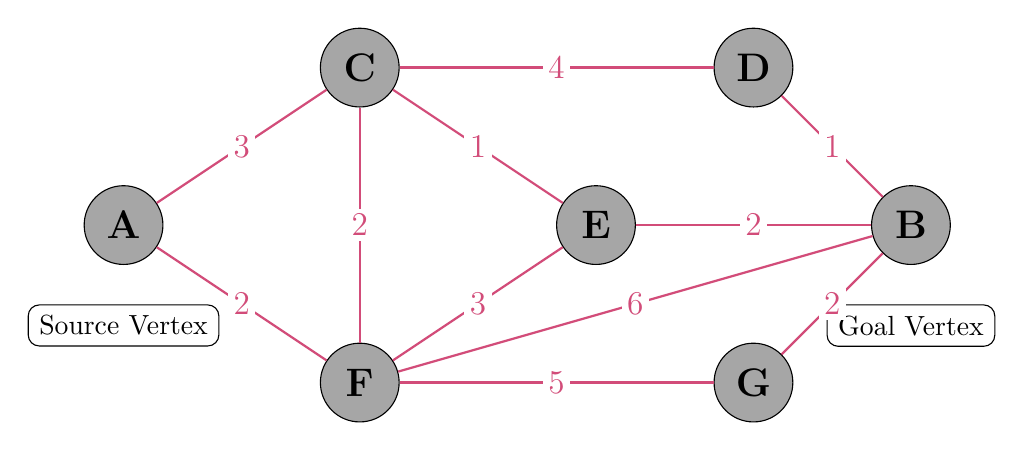
\begin{tikzpicture}[
    node distance=3cm,
    vertex/.style={circle, draw, fill=gray!70, minimum size=1cm, font=\Large\bfseries},
    edge/.style={draw, thick, color=purple!70},
    weight/.style={fill=white, inner sep=2pt, font=\large}
]

% Define node positions
\node[vertex] (A) at (-4, 0) {A};
\node[vertex] (C) at (-1, 2) {C};
\node[vertex] (F) at (-1, -2) {F};
\node[vertex] (E) at (2, 0) {E};
\node[vertex] (D) at (4, 2) {D};
\node[vertex] (B) at (6, 0) {B};
\node[vertex] (G) at (4, -2) {G};

% Add source vertex label
\node[below=0.5cm of A, draw, fill=white, rounded corners, inner sep=4pt] {Source Vertex};

% Add goal vertex label
\node[below=0.5cm of B, draw, fill=white, rounded corners, inner sep=4pt] {Goal Vertex};

% Draw edges with weights
\draw[edge] (A) -- (C) node[weight, midway] {3};
\draw[edge] (A) -- (F) node[weight, midway] {2};
\draw[edge] (C) -- (D) node[weight, midway] {4};
\draw[edge] (C) -- (E) node[weight, midway] {1};
\draw[edge] (C) -- (F) node[weight, midway] {2};
\draw[edge] (E) -- (F) node[weight, midway] {3};
\draw[edge] (E) -- (B) node[weight, midway] {2};
\draw[edge] (F) -- (B) node[weight, midway] {6};
\draw[edge] (D) -- (B) node[weight, midway] {1};
\draw[edge] (B) -- (G) node[weight, midway] {2};
\draw[edge] (F) -- (G) node[weight, midway] {5};

\end{tikzpicture}
\end{center}
% ----------- PICTURE 2 ----------
\subsection{Algorithm Initialization}
\begin{center}
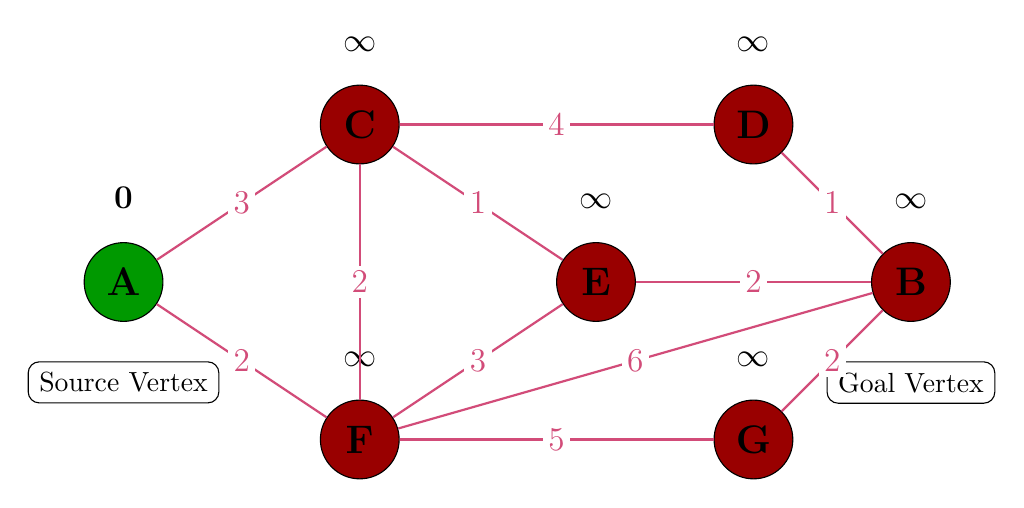
\begin{tikzpicture}[
    node distance=3cm,
    vertex/.style={circle, draw, fill=gray!70, minimum size=1cm, font=\Large\bfseries},
    edge/.style={draw, thick, color=purple!70},
    weight/.style={fill=white, inner sep=2pt, font=\large}
]

% Define node positions
\node[vertex, fill=green!60!black] (A) at (-4, 0) {A};
\node[vertex, fill=red!60!black] (C) at (-1, 2) {C};
\node[vertex, fill=red!60!black] (F) at (-1, -2) {F};
\node[vertex, fill=red!60!black] (E) at (2, 0) {E};
\node[vertex, fill=red!60!black] (D) at (4, 2) {D};
\node[vertex, fill=red!60!black] (B) at (6, 0) {B};
\node[vertex, fill=red!60!black] (G) at (4, -2) {G};

% Add distance labels above vertices
\node[above=0.3cm of A, font=\large\bfseries] {0};
\node[above=0.3cm of C, font=\large\bfseries] {$\infty$};
\node[above=0.3cm of F, font=\large\bfseries] {$\infty$};
\node[above=0.3cm of E, font=\large\bfseries] {$\infty$};
\node[above=0.3cm of D, font=\large\bfseries] {$\infty$};
\node[above=0.3cm of B, font=\large\bfseries] {$\infty$};
\node[above=0.3cm of G, font=\large\bfseries] {$\infty$};

% Add source vertex label
\node[below=0.5cm of A, draw, fill=white, rounded corners, inner sep=4pt] {Source Vertex};

% Add goal vertex label
\node[below=0.5cm of B, draw, fill=white, rounded corners, inner sep=4pt] {Goal Vertex};

% Draw edges with weights
\draw[edge] (A) -- (C) node[weight, midway] {3};
\draw[edge] (A) -- (F) node[weight, midway] {2};
\draw[edge] (C) -- (D) node[weight, midway] {4};
\draw[edge] (C) -- (E) node[weight, midway] {1};
\draw[edge] (C) -- (F) node[weight, midway] {2};
\draw[edge] (E) -- (F) node[weight, midway] {3};
\draw[edge] (E) -- (B) node[weight, midway] {2};
\draw[edge] (F) -- (B) node[weight, midway] {6};
\draw[edge] (D) -- (B) node[weight, midway] {1};
\draw[edge] (B) -- (G) node[weight, midway] {2};
\draw[edge] (F) -- (G) node[weight, midway] {5};

\end{tikzpicture}
\end{center}

% ----------- PICTURE 3 ----------
\subsection{Processing Source Vertex A}
\begin{center}
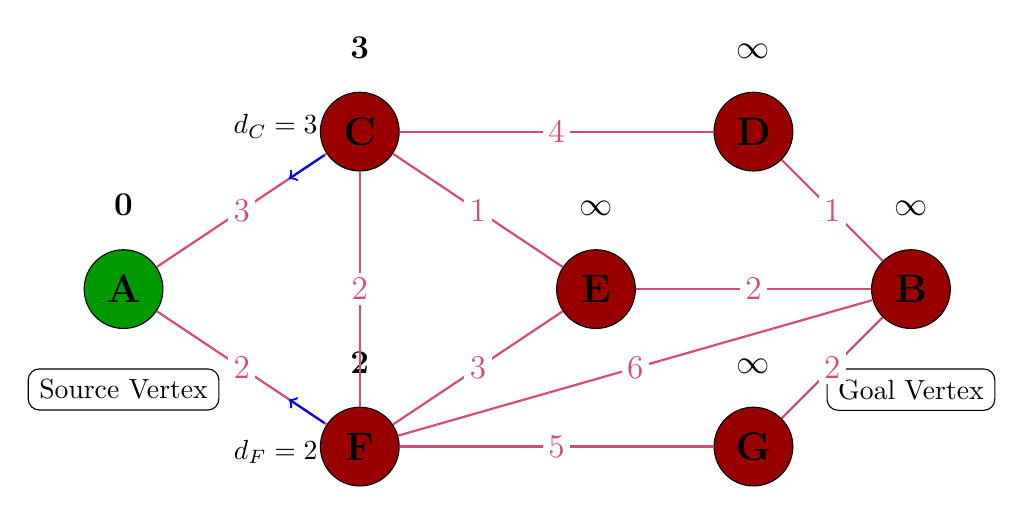
\begin{tikzpicture}[
    node distance=3cm,
    vertex/.style={circle, draw, fill=gray!70, minimum size=1cm, font=\Large\bfseries},
    edge/.style={draw, thick, color=purple!70},
    weight/.style={fill=white, inner sep=2pt, font=\large}
]

% Define node positions
\node[vertex, fill=green!60!black] (A) at (-4, 0) {A};
\node[vertex, fill=red!60!black] (C) at (-1, 2) {C};
\node[vertex, fill=red!60!black] (F) at (-1, -2) {F};
\node[vertex, fill=red!60!black] (E) at (2, 0) {E};
\node[vertex, fill=red!60!black] (D) at (4, 2) {D};
\node[vertex, fill=red!60!black] (B) at (6, 0) {B};
\node[vertex, fill=red!60!black] (G) at (4, -2) {G};

% Add distance labels above vertices
\node[above=0.3cm of A, font=\large\bfseries] {0};
\node[above=0.3cm of C, font=\large\bfseries] {3};
\node[above=0.3cm of F, font=\large\bfseries] {2};
\node[above=0.3cm of E, font=\large\bfseries] {$\infty$};
\node[above=0.3cm of D, font=\large\bfseries] {$\infty$};
\node[above=0.3cm of B, font=\large\bfseries] {$\infty$};
\node[above=0.3cm of G, font=\large\bfseries] {$\infty$};

% Add source vertex label
\node[below=0.5cm of A, draw, fill=white, rounded corners, inner sep=4pt] {Source Vertex};

% Add goal vertex label
\node[below=0.5cm of B, draw, fill=white, rounded corners, inner sep=4pt] {Goal Vertex};

% Draw edges with weights
\draw[edge] (A) -- (C) node[weight, midway] {3} node[pos=0.7, above=5mm, color=black] {$d_C = 3$};
\draw[edge] (A) -- (F) node[weight, midway] {2} node[pos=0.7, below=5mm, color=black] {$d_F = 2$};
\draw[edge] (C) -- (D) node[weight, midway] {4};
\draw[edge] (C) -- (E) node[weight, midway] {1};
\draw[edge] (C) -- (F) node[weight, midway] {2};
\draw[edge] (E) -- (F) node[weight, midway] {3};
\draw[edge] (E) -- (B) node[weight, midway] {2};
\draw[edge] (F) -- (B) node[weight, midway] {6};
\draw[edge] (D) -- (B) node[weight, midway] {1};
\draw[edge] (B) -- (G) node[weight, midway] {2};
\draw[edge] (F) -- (G) node[weight, midway] {5};

% Blue arrows for Picture 3 (pointing from child to parent)
\draw[->, blue, thick] ($ (C)!0.15!(A) $) -- ($ (C)!0.3!(A) $);
\draw[->, blue, thick] ($ (F)!0.15!(A) $) -- ($ (F)!0.3!(A) $);

\end{tikzpicture}
\end{center}

% ----------- PICTURE 4 ----------
\subsection{Processing Vertex F}
\begin{center}
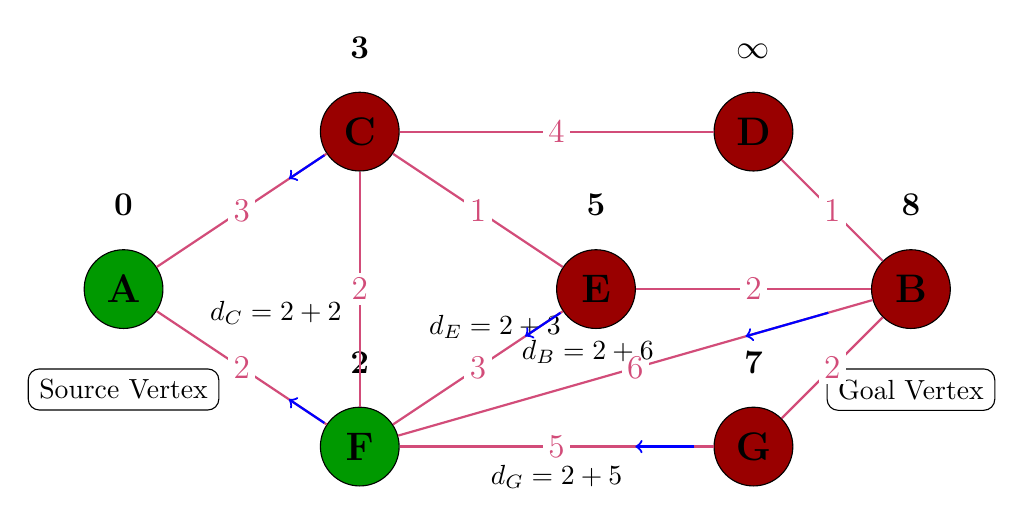
\begin{tikzpicture}[
    node distance=3cm,
    vertex/.style={circle, draw, fill=gray!70, minimum size=1cm, font=\Large\bfseries},
    edge/.style={draw, thick, color=purple!70},
    weight/.style={fill=white, inner sep=2pt, font=\large}
]

% Define node positions
\node[vertex, fill=green!60!black] (A) at (-4, 0) {A};
\node[vertex, fill=red!60!black] (C) at (-1, 2) {C};
\node[vertex, fill=green!60!black] (F) at (-1, -2) {F};
\node[vertex, fill=red!60!black] (E) at (2, 0) {E};
\node[vertex, fill=red!60!black] (D) at (4, 2) {D};
\node[vertex, fill=red!60!black] (B) at (6, 0) {B};
\node[vertex, fill=red!60!black] (G) at (4, -2) {G};

% Add distance labels above vertices
\node[above=0.3cm of A, font=\large\bfseries] {0};
\node[above=0.3cm of C, font=\large\bfseries] {3};
\node[above=0.3cm of F, font=\large\bfseries] {2};
\node[above=0.3cm of E, font=\large\bfseries] {5};
\node[above=0.3cm of D, font=\large\bfseries] {$\infty$};
\node[above=0.3cm of B, font=\large\bfseries] {8};
\node[above=0.3cm of G, font=\large\bfseries] {7};

% Add source vertex label
\node[below=0.5cm of A, draw, fill=white, rounded corners, inner sep=4pt] {Source Vertex};

% Add goal vertex label
\node[below=0.5cm of B, draw, fill=white, rounded corners, inner sep=4pt] {Goal Vertex};

% Draw edges with weights and distance calculations
\draw[edge] (A) -- (C) node[weight, midway] {3};
\draw[edge] (A) -- (F) node[weight, midway] {2};
\draw[edge] (C) -- (D) node[weight, midway] {4};
\draw[edge] (C) -- (E) node[weight, midway] {1};
\draw[edge] (C) -- (F) node[weight, midway] {2} node[pos=0.6, left=1mm, color=black] {$d_C = 2 + 2$};
\draw[edge] (E) -- (F) node[weight, midway] {3} node[pos=0.4, above=1mm, color=black] {$d_E = 2 + 3$};
\draw[edge] (E) -- (B) node[weight, midway] {2};
\draw[edge] (F) -- (B) node[weight, midway] {6} node[pos=0.4, above=1mm, color=black] {$d_B = 2 + 6$};
\draw[edge] (D) -- (B) node[weight, midway] {1};
\draw[edge] (B) -- (G) node[weight, midway] {2};
\draw[edge] (F) -- (G) node[weight, midway] {5} node[pos=0.5, below=1mm, color=black] {$d_G = 2 + 5$};

% Blue arrows for Picture 4 (pointing from child to parent)
\draw[->, blue, thick] ($ (E)!0.15!(F) $) -- ($ (E)!0.3!(F) $);
\draw[->, blue, thick] ($ (B)!0.15!(F) $) -- ($ (B)!0.3!(F) $);
\draw[->, blue, thick] ($ (G)!0.15!(F) $) -- ($ (G)!0.3!(F) $);
\draw[->, blue, thick] ($ (C)!0.15!(A) $) -- ($ (C)!0.3!(A) $);
\draw[->, blue, thick] ($ (F)!0.15!(A) $) -- ($ (F)!0.3!(A) $);

\end{tikzpicture}
\end{center}

% ----------- PICTURE 5 ----------
\subsection{Processing Vertex C}
\begin{center}
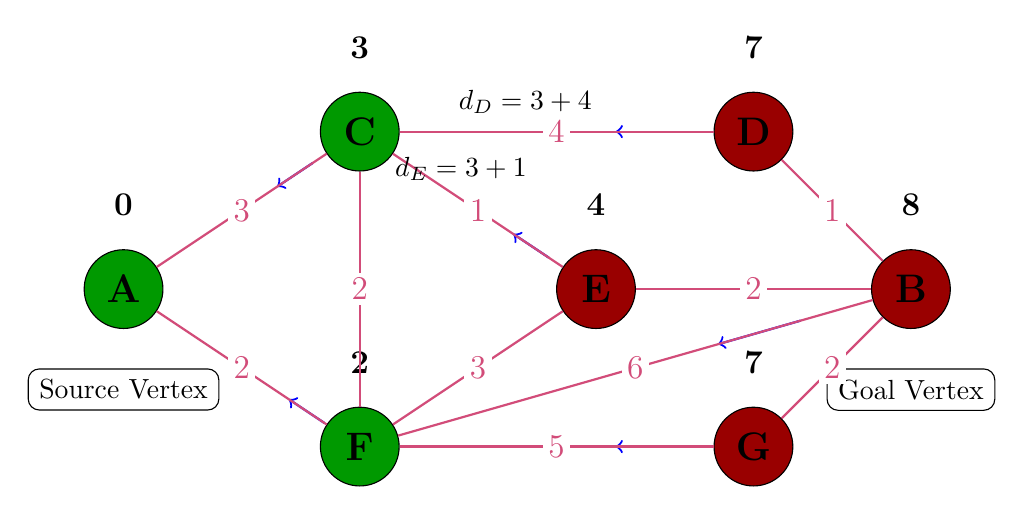
\begin{tikzpicture}[
    node distance=3cm,
    vertex/.style={circle, draw, fill=gray!70, minimum size=1cm, font=\Large\bfseries},
    edge/.style={draw, thick, color=purple!70},
    weight/.style={fill=white, inner sep=2pt, font=\large}
]

% Define node positions
\node[vertex, fill=green!60!black] (A) at (-4, 0) {A};
\node[vertex, fill=green!60!black] (C) at (-1, 2) {C};
\node[vertex, fill=green!60!black] (F) at (-1, -2) {F};
\node[vertex, fill=red!60!black] (E) at (2, 0) {E};
\node[vertex, fill=red!60!black] (D) at (4, 2) {D};
\node[vertex, fill=red!60!black] (B) at (6, 0) {B};
\node[vertex, fill=red!60!black] (G) at (4, -2) {G};

% Blue arrows for Picture 5 (pointing from child to parent)
\draw[->, blue, thick] ($ (E)!0.2!(C) $) -- ($ (E)!0.35!(C) $);
\draw[->, blue, thick] ($ (D)!0.2!(C) $) -- ($ (D)!0.35!(C) $);
\draw[->, blue, thick] ($ (B)!0.2!(F) $) -- ($ (B)!0.35!(F) $);
\draw[->, blue, thick] ($ (G)!0.2!(F) $) -- ($ (G)!0.35!(F) $);
\draw[->, blue, thick] ($ (C)!0.2!(A) $) -- ($ (C)!0.35!(A) $);
\draw[->, blue, thick] ($ (F)!0.15!(A) $) -- ($ (F)!0.3!(A) $);

% Add distance labels above vertices
\node[above=0.3cm of A, font=\large\bfseries] {0};
\node[above=0.3cm of C, font=\large\bfseries] {3};
\node[above=0.3cm of F, font=\large\bfseries] {2};
\node[above=0.3cm of E, font=\large\bfseries] {4};
\node[above=0.3cm of D, font=\large\bfseries] {7};
\node[above=0.3cm of B, font=\large\bfseries] {8};
\node[above=0.3cm of G, font=\large\bfseries] {7};

% Add source vertex label
\node[below=0.5cm of A, draw, fill=white, rounded corners, inner sep=4pt] {Source Vertex};

% Add goal vertex label
\node[below=0.5cm of B, draw, fill=white, rounded corners, inner sep=4pt] {Goal Vertex};

% Draw edges with weights and distance calculations
\draw[edge] (A) -- (C) node[weight, midway] {3};
\draw[edge] (A) -- (F) node[weight, midway] {2};
\draw[edge] (C) -- (D) node[weight, midway] {4} node[pos=0.4, above=1mm, color=black] {$d_D = 3 + 4$};
\draw[edge] (C) -- (E) node[weight, midway] {1} node[pos=0.4, above=1mm, color=black] {$d_E = 3 + 1$};
\draw[edge] (C) -- (F) node[weight, midway] {2};
\draw[edge] (E) -- (F) node[weight, midway] {3};
\draw[edge] (E) -- (B) node[weight, midway] {2};
\draw[edge] (F) -- (B) node[weight, midway] {6};
\draw[edge] (D) -- (B) node[weight, midway] {1};
\draw[edge] (B) -- (G) node[weight, midway] {2};
\draw[edge] (F) -- (G) node[weight, midway] {5};

\end{tikzpicture}
\end{center}

% ----------- PICTURE 6 ----------
\subsection{Processing Vertex E}
\begin{center}
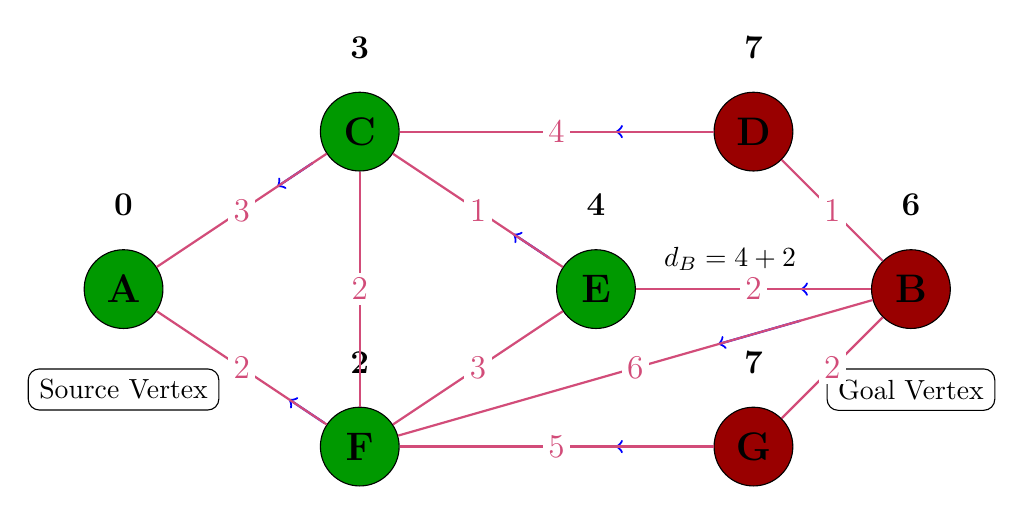
\begin{tikzpicture}[
    node distance=3cm,
    vertex/.style={circle, draw, fill=gray!70, minimum size=1cm, font=\Large\bfseries},
    edge/.style={draw, thick, color=purple!70},
    weight/.style={fill=white, inner sep=2pt, font=\large}
]

% Define node positions
\node[vertex, fill=green!60!black] (A) at (-4, 0) {A};
\node[vertex, fill=green!60!black] (C) at (-1, 2) {C};
\node[vertex, fill=green!60!black] (F) at (-1, -2) {F};
\node[vertex, fill=green!60!black] (E) at (2, 0) {E};
\node[vertex, fill=red!60!black] (D) at (4, 2) {D};
\node[vertex, fill=red!60!black] (B) at (6, 0) {B};
\node[vertex, fill=red!60!black] (G) at (4, -2) {G};

% Blue arrows for Picture 6 (pointing from child to parent)
\draw[->, blue, thick] ($ (D)!0.2!(C) $) -- ($ (D)!0.35!(C) $);
\draw[->, blue, thick] ($ (B)!0.2!(E) $) -- ($ (B)!0.35!(E) $);
\draw[->, blue, thick] ($ (G)!0.2!(F) $) -- ($ (G)!0.35!(F) $);
\draw[->, blue, thick] ($ (C)!0.2!(A) $) -- ($ (C)!0.35!(A) $);
\draw[->, blue, thick] ($ (E)!0.2!(C) $) -- ($ (E)!0.35!(C) $);
\draw[->, blue, thick] ($ (F)!0.15!(A) $) -- ($ (F)!0.3!(A) $);
\draw[->, blue, thick] ($ (B)!0.2!(F) $) -- ($ (B)!0.35!(F) $);

% Add distance labels above vertices
\node[above=0.3cm of A, font=\large\bfseries] {0};
\node[above=0.3cm of C, font=\large\bfseries] {3};
\node[above=0.3cm of F, font=\large\bfseries] {2};
\node[above=0.3cm of E, font=\large\bfseries] {4};
\node[above=0.3cm of D, font=\large\bfseries] {7};
\node[above=0.3cm of B, font=\large\bfseries] {6};
\node[above=0.3cm of G, font=\large\bfseries] {7};

% Add source vertex label
\node[below=0.5cm of A, draw, fill=white, rounded corners, inner sep=4pt] {Source Vertex};

% Add goal vertex label
\node[below=0.5cm of B, draw, fill=white, rounded corners, inner sep=4pt] {Goal Vertex};

% Draw edges with weights and distance calculations
\draw[edge] (A) -- (C) node[weight, midway] {3};
\draw[edge] (A) -- (F) node[weight, midway] {2};
\draw[edge] (C) -- (D) node[weight, midway] {4};
\draw[edge] (C) -- (E) node[weight, midway] {1};
\draw[edge] (C) -- (F) node[weight, midway] {2};
\draw[edge] (E) -- (F) node[weight, midway] {3};
\draw[edge] (E) -- (B) node[weight, midway] {2} node[pos=0.4, above=1mm, color=black] {$d_B = 4 + 2$};
\draw[edge] (F) -- (B) node[weight, midway] {6};
\draw[edge] (D) -- (B) node[weight, midway] {1};
\draw[edge] (B) -- (G) node[weight, midway] {2};
\draw[edge] (F) -- (G) node[weight, midway] {5};

\end{tikzpicture}
\end{center}

% ----------- PICTURE 7 ----------
\subsection{Processing Vertex B}
\begin{center}
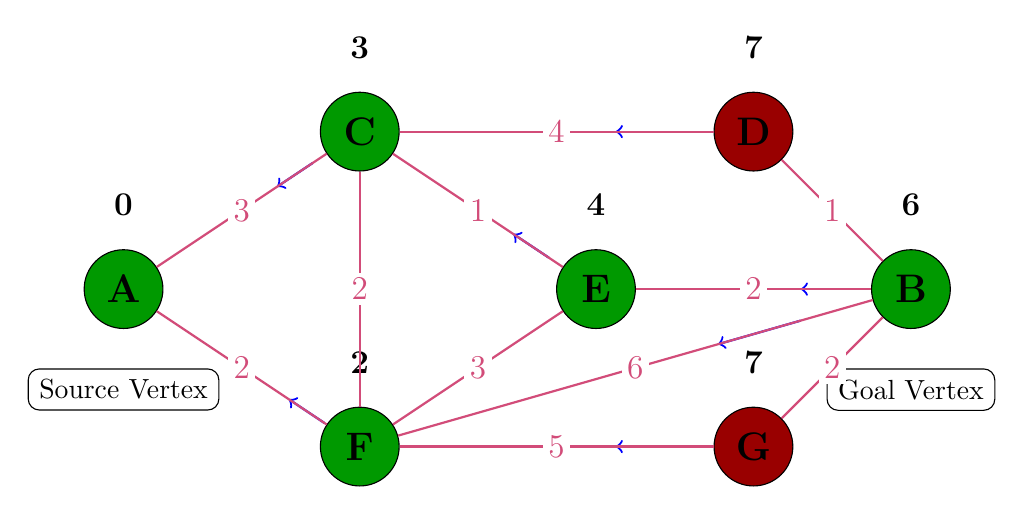
\begin{tikzpicture}[
    node distance=3cm,
    vertex/.style={circle, draw, fill=gray!70, minimum size=1cm, font=\Large\bfseries},
    edge/.style={draw, thick, color=purple!70},
    weight/.style={fill=white, inner sep=2pt, font=\large}
]

% Define node positions
\node[vertex, fill=green!60!black] (A) at (-4, 0) {A};
\node[vertex, fill=green!60!black] (C) at (-1, 2) {C};
\node[vertex, fill=green!60!black] (F) at (-1, -2) {F};
\node[vertex, fill=green!60!black] (E) at (2, 0) {E};
\node[vertex, fill=red!60!black] (D) at (4, 2) {D};
\node[vertex, fill=green!60!black] (B) at (6, 0) {B};
\node[vertex, fill=red!60!black] (G) at (4, -2) {G};

% Blue arrows for Picture 7 (pointing from child to parent)
\draw[->, blue, thick] ($ (D)!0.2!(C) $) -- ($ (D)!0.35!(C) $);
\draw[->, blue, thick] ($ (G)!0.2!(F) $) -- ($ (G)!0.35!(F) $);
\draw[->, blue, thick] ($ (C)!0.2!(A) $) -- ($ (C)!0.35!(A) $);
\draw[->, blue, thick] ($ (E)!0.2!(C) $) -- ($ (E)!0.35!(C) $);
\draw[->, blue, thick] ($ (B)!0.2!(E) $) -- ($ (B)!0.35!(E) $);
\draw[->, blue, thick] ($ (F)!0.15!(A) $) -- ($ (F)!0.3!(A) $);
\draw[->, blue, thick] ($ (B)!0.2!(F) $) -- ($ (B)!0.35!(F) $);

% Add distance labels above vertices
\node[above=0.3cm of A, font=\large\bfseries] {0};
\node[above=0.3cm of C, font=\large\bfseries] {3};
\node[above=0.3cm of F, font=\large\bfseries] {2};
\node[above=0.3cm of E, font=\large\bfseries] {4};
\node[above=0.3cm of D, font=\large\bfseries] {7};
\node[above=0.3cm of B, font=\large\bfseries] {6};
\node[above=0.3cm of G, font=\large\bfseries] {7};

% Add source vertex label
\node[below=0.5cm of A, draw, fill=white, rounded corners, inner sep=4pt] {Source Vertex};

% Add goal vertex label
\node[below=0.5cm of B, draw, fill=white, rounded corners, inner sep=4pt] {Goal Vertex};

% Draw edges with weights
\draw[edge] (A) -- (C) node[weight, midway] {3};
\draw[edge] (A) -- (F) node[weight, midway] {2};
\draw[edge] (C) -- (D) node[weight, midway] {4};
\draw[edge] (C) -- (E) node[weight, midway] {1};
\draw[edge] (C) -- (F) node[weight, midway] {2};
\draw[edge] (E) -- (F) node[weight, midway] {3};
\draw[edge] (E) -- (B) node[weight, midway] {2};
\draw[edge] (F) -- (B) node[weight, midway] {6};
\draw[edge] (D) -- (B) node[weight, midway] {1};
\draw[edge] (B) -- (G) node[weight, midway] {2};
\draw[edge] (F) -- (G) node[weight, midway] {5};

\end{tikzpicture}
\end{center}

% ----------- PICTURE 8 ----------
\subsection{Shortest Path from B to A}
\begin{center}
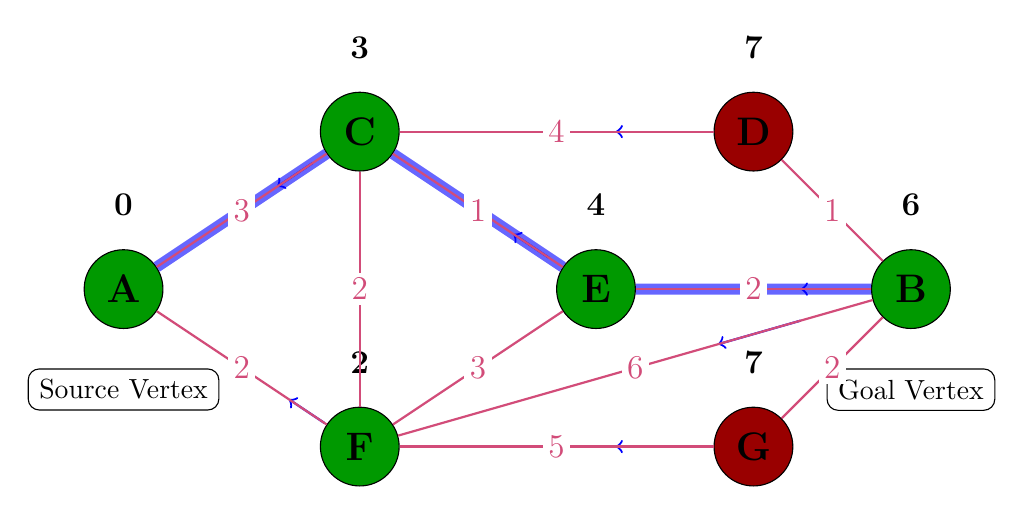
\begin{tikzpicture}[
    node distance=3cm,
    vertex/.style={circle, draw, fill=gray!70, minimum size=1cm, font=\Large\bfseries},
    edge/.style={draw, thick, color=purple!70},
    weight/.style={fill=white, inner sep=2pt, font=\large}
]

% Define node positions
\node[vertex, fill=green!60!black] (A) at (-4, 0) {A};
\node[vertex, fill=green!60!black] (C) at (-1, 2) {C};
\node[vertex, fill=green!60!black] (F) at (-1, -2) {F};
\node[vertex, fill=green!60!black] (E) at (2, 0) {E};
\node[vertex, fill=red!60!black] (D) at (4, 2) {D};
\node[vertex, fill=green!60!black] (B) at (6, 0) {B};
\node[vertex, fill=red!60!black] (G) at (4, -2) {G};

% Blue arrows for Picture 8 (pointing from child to parent)
\draw[->, blue, thick] ($ (D)!0.2!(C) $) -- ($ (D)!0.35!(C) $);
\draw[->, blue, thick] ($ (G)!0.2!(F) $) -- ($ (G)!0.35!(F) $);
\draw[->, blue, thick] ($ (C)!0.2!(A) $) -- ($ (C)!0.35!(A) $);
\draw[->, blue, thick] ($ (E)!0.2!(C) $) -- ($ (E)!0.35!(C) $);
\draw[->, blue, thick] ($ (B)!0.2!(E) $) -- ($ (B)!0.35!(E) $);
\draw[->, blue, thick] ($ (F)!0.15!(A) $) -- ($ (F)!0.3!(A) $);
\draw[->, blue, thick] ($ (B)!0.2!(F) $) -- ($ (B)!0.35!(F) $);

% Shortest path from B to A (thick partially transparent blue line)
\draw[blue, line width=4pt, opacity=0.6] (B) -- (E) -- (C) -- (A);

% Add distance labels above vertices
\node[above=0.3cm of A, font=\large\bfseries] {0};
\node[above=0.3cm of C, font=\large\bfseries] {3};
\node[above=0.3cm of F, font=\large\bfseries] {2};
\node[above=0.3cm of E, font=\large\bfseries] {4};
\node[above=0.3cm of D, font=\large\bfseries] {7};
\node[above=0.3cm of B, font=\large\bfseries] {6};
\node[above=0.3cm of G, font=\large\bfseries] {7};

% Add source vertex label
\node[below=0.5cm of A, draw, fill=white, rounded corners, inner sep=4pt] {Source Vertex};

% Add goal vertex label
\node[below=0.5cm of B, draw, fill=white, rounded corners, inner sep=4pt] {Goal Vertex};

% Draw edges with weights
\draw[edge] (A) -- (C) node[weight, midway] {3};
\draw[edge] (A) -- (F) node[weight, midway] {2};
\draw[edge] (C) -- (D) node[weight, midway] {4};
\draw[edge] (C) -- (E) node[weight, midway] {1};
\draw[edge] (C) -- (F) node[weight, midway] {2};
\draw[edge] (E) -- (F) node[weight, midway] {3};
\draw[edge] (E) -- (B) node[weight, midway] {2};
\draw[edge] (F) -- (B) node[weight, midway] {6};
\draw[edge] (D) -- (B) node[weight, midway] {1};
\draw[edge] (B) -- (G) node[weight, midway] {2};
\draw[edge] (F) -- (G) node[weight, midway] {5};

\end{tikzpicture}
\end{center}

\end{document}